\section{Einführung und Definitionen}

\begin{frame}
    \begin{block}{Themenvorstellung}
        \begin{itemize}
            \item Analyse boolscher Funktionen über das Konzept der Rechtecke
            \item Untere Schranke für die Blattgröße DeMorgan'scher Formeln
            \item Generalisierte Komplexitätsmaße:
                \begin{itemize}
                    \item konvexe Maße
                    \item submodulare Maße
                \end{itemize}
        \end{itemize}
    \end{block}
\end{frame}

\begin{frame}{Wiederholung}
    \begin{block}{Definition [DeMorgan-Schaltkreis]}
        \begin{itemize}
            \item $\Phi := \{ \wedge, \vee, \neg \}$ boolsche Basis
            \item $\neg\ $-Gatter nur bei Inputvariablen
        \end{itemize}
        
        %Sei $\Phi := \{ \wedge, \vee, \neg \}$ eine boolsche Basis.\\
        %Ein DeMorgan-Schaltkreis ist ein Schaltkreis über der Basis %$\Phi$, wobei die $\neg\ $-Gatter nur bei Inputvariablen %angewendet wird.
        
    \end{block}
    \begin{block}{Definition [Formel, Blattgröße]}
        \begin{itemize}
            \item boolsche Funktion f
            \item Fan-Out 1 Schaltkreis
            \item $L(f)$ ist die Anzahl der Eingabegatter
        \end{itemize}
        
        %Eine boolsche Formel $f$ ist ein Schaltkreis mit Fan-Out %$1$.\\
        %Die Blattgröße $L(f)$ beschreibt die Anzahl der %Eingabegatter.
        
    \end{block}
\end{frame}

\begin{frame}
    \begin{block}{Definition [kombinatorisches Rechteck]}
        \begin{itemize}
            \item $R = A \times B$, $A, B \subset \{0, 1\}^n $ disjunkt
            \item $S\subset R$ Unterrechteck, falls $S$ ebenfalls ein Rechteck ist
        \end{itemize}
        
        %Ein n-dimensionales kombinatorisches Rechteck ist ein %karthesisches Produkt $R = A \times B$, wobei $A, B \subset %\{0, 1\}^n$ und disjunkt sind.
        %\newline
        %$S \subset R$ ist Unterrechteck, falls $S$ ebenfalls ein %Rechteck ist.
    \end{block}
    
    \begin{block}{Bemerkung}
        \begin{itemize}
            \item $R$ ist bipartiter Graph.
            \item $(a,b) \in R$ sind Paare von Ecken.
        \end{itemize}
    \end{block}
\end{frame}

\begin{frame}
    \begin{figure}
        \centering
        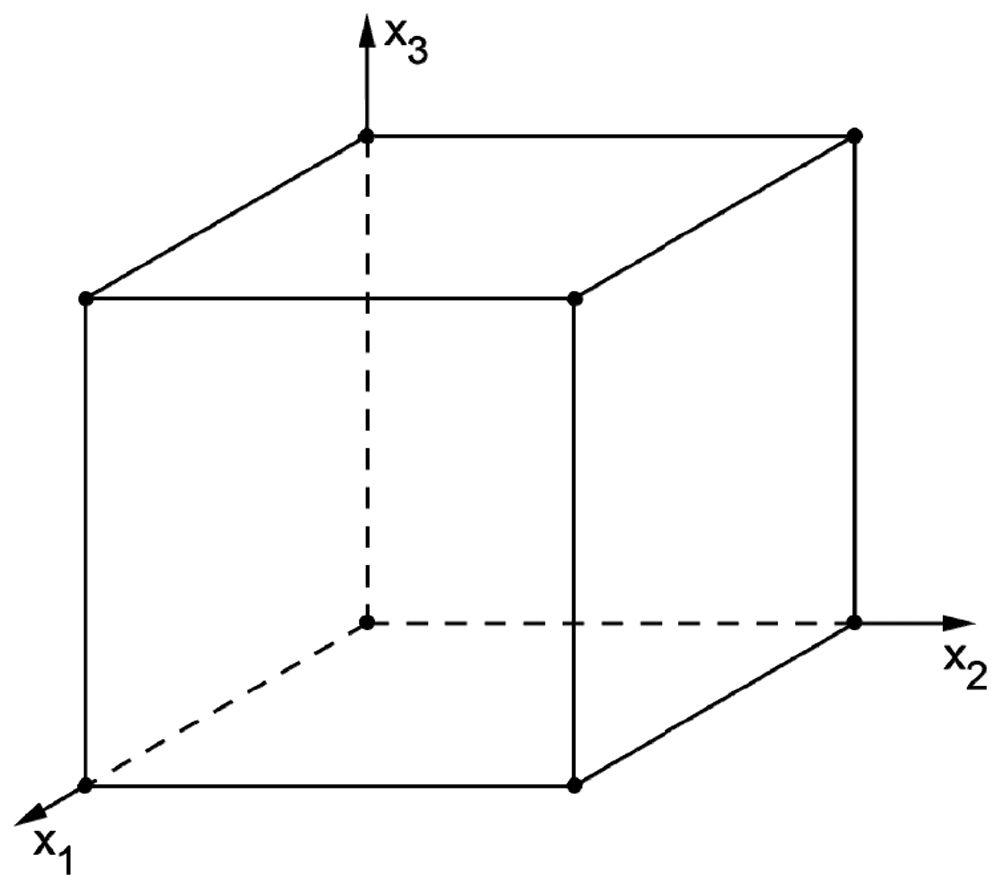
\includegraphics[width=80mm,scale=0.5]{wuerfel.png}
        \caption{Beispiel}
    \end{figure}
\end{frame}

\begin{frame}
    \begin{block}{Definition}
        Sei $f$ eine boolsche Funktion und $R = A \times B$ ein Rechteck. $f$ separiert $R$, falls $f(A) = 1, f(B) = 0$.
        \newline
        \newline
        Dabei ist
        \[ 
            f(A) = 1 \Leftrightarrow \forall a \in A : f(a) = 1
        \] 
        \[
            f(B) = 0 \Leftrightarrow \forall b \in B : f(b) = 0
        \]
    \end{block}
\end{frame}

\begin{frame}
    \begin{block}{Definition}
        Ein Rechteck $R = A\times B$ heißt monochrom, wenn ein Index $i$ existiert, so dass
        \newline
        \[ 
            a_i \neq b_i \text{ für alle Kanten } (a,b) \in R 
        \]
        Analog ist $R$ positiv monochrom, wenn
        \[
            a_i = 1,\ b_i = 0\ \text{für alle Kanten } (a,b) \in R
        \]
    \end{block}
\end{frame}

\begin{frame}
    \begin{figure}
        \centering
        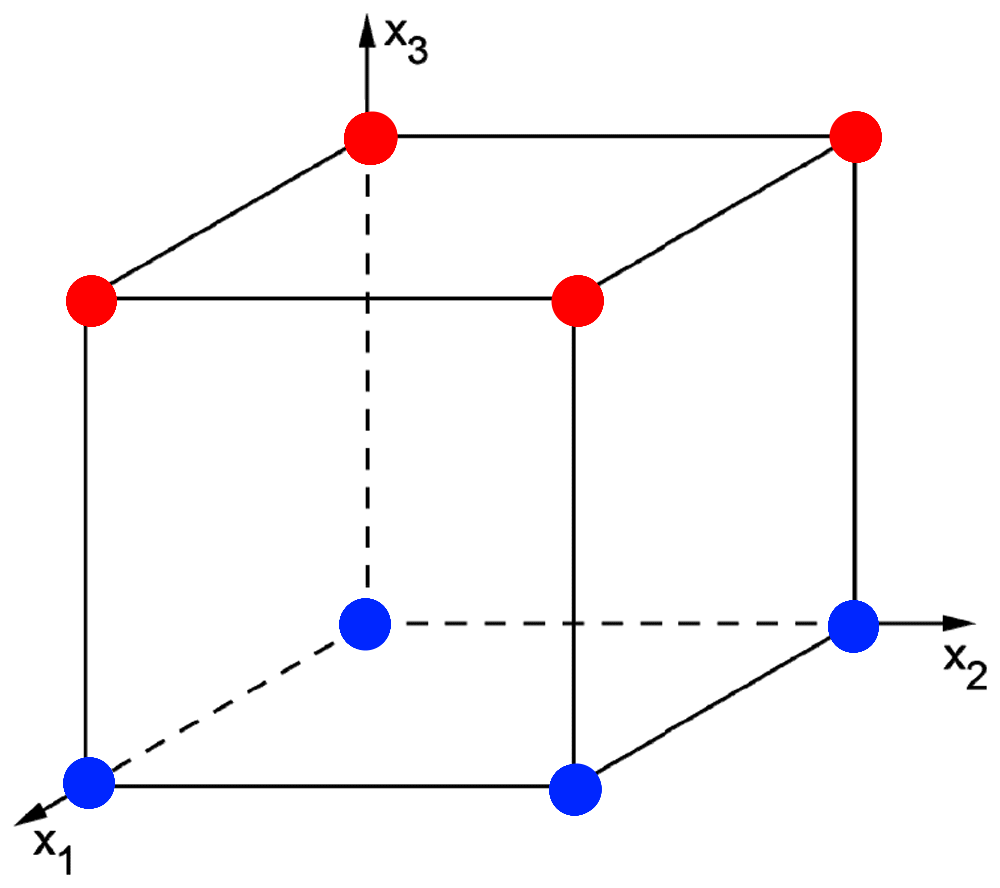
\includegraphics[width=80mm,scale=0.5]{monochrom1.png}
        \caption{(positiv) monochromes Rechteck}
    \end{figure}
\end{frame}

\begin{frame}
    \begin{figure}
        \centering
        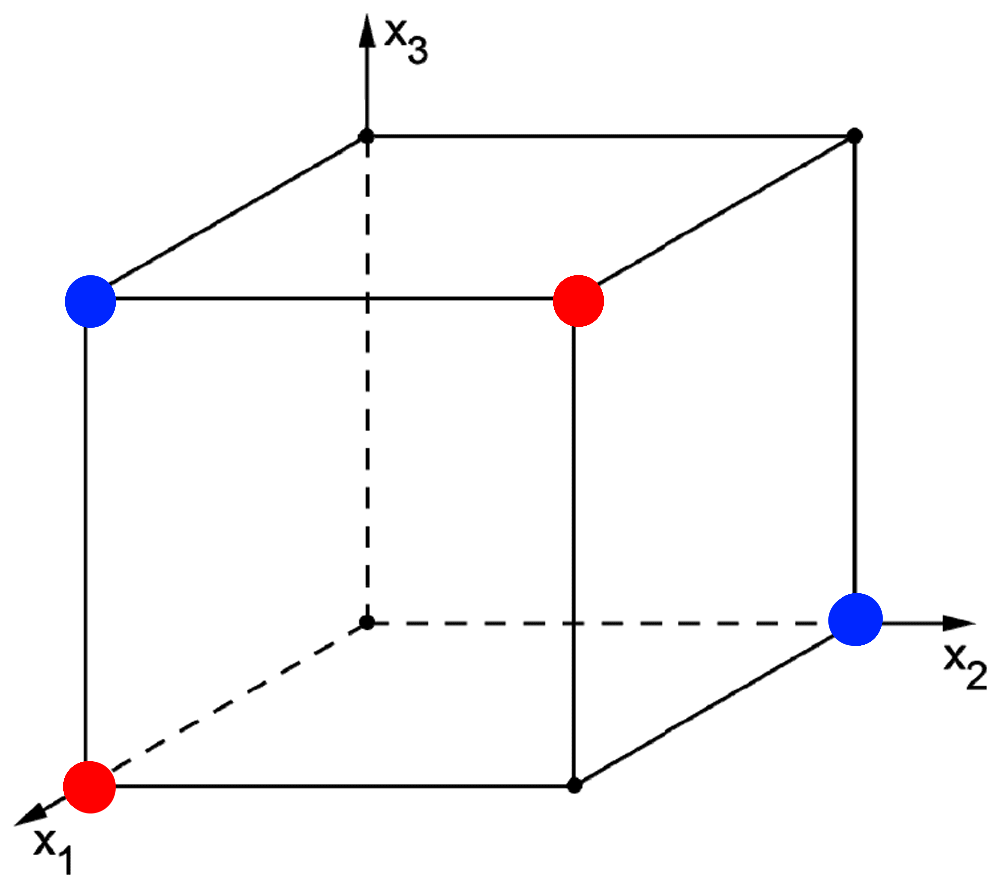
\includegraphics[width=80mm,scale=0.5]{monochrom2.png}
        \caption{nichtmonochromes Rechteck}
    \end{figure}
\end{frame}

\begin{frame}
    \begin{figure}
        \centering
        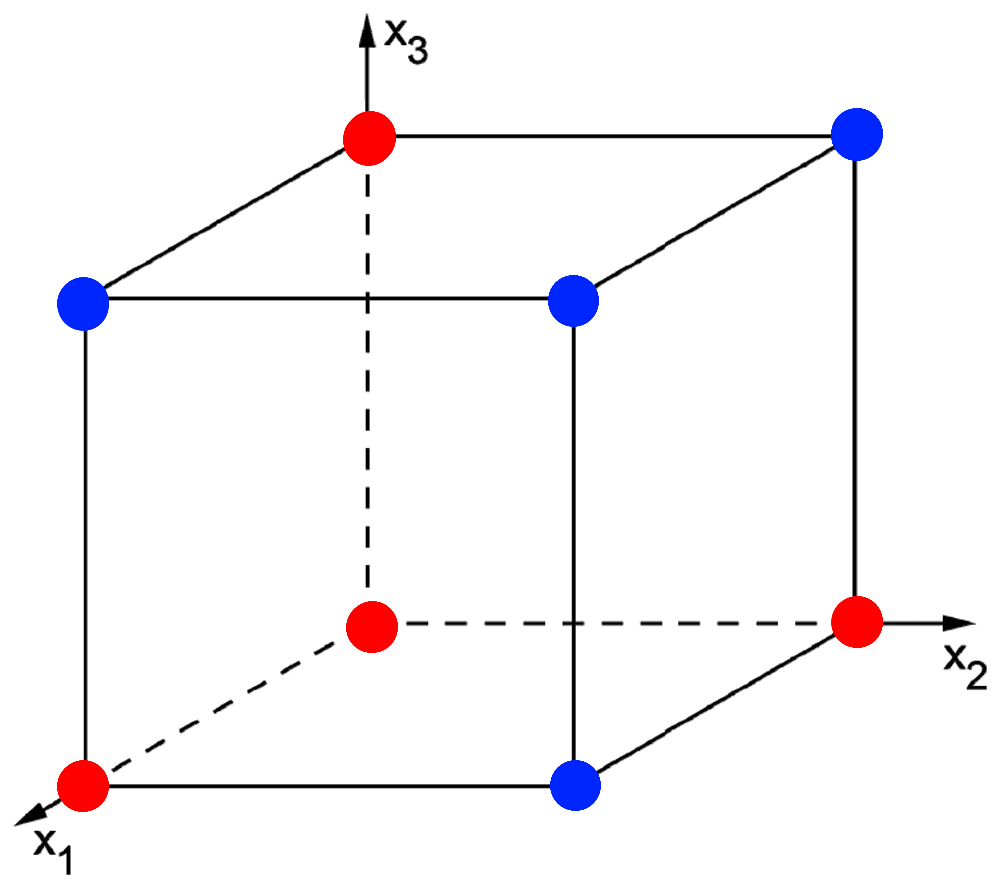
\includegraphics[width=80mm,scale=0.5]{monochrom3.png}
        \caption{nichtmonochromes Rechteck}
    \end{figure}
\end{frame}

\begin{frame}
    \begin{block}{Definition [Partitionszahl]}
        \begin{itemize}
            \item $R$ Rechteck, $f$ boolsche Funktion
            \item $\chi(R)$ Partitionszahl
            \item Größe der kleinsten Partition in \textbf{disjunkte} monochrome Rechtecke
            \item $\chi_+(R)$ analog für positiv monochrome Rechtecke
            \item $\chi (f) := \chi (f^{-1}(1) \times f^{-1}(0))$
        \end{itemize}
        
        %Sei $R$ ein Rechteck. Die Partitionszahl $\chi (R)$ ist die %kleinste Zahl $t$, so dass sich $R$ in $t$ \textbf{disjunkte}
        %monochrome Rechtecke separieren lässt.
        %\newline
        %\newline
        %Analog für positive monochrome Rechtecke ist die positive %Partitionszahl $\chi_+(R)$ definiert, falls sie existiert.
    \end{block}
\end{frame}

%%%%%%%%%%%%%%%%%%%%%%%%%%%%%%%%%%%%%%%%%%%%%%%%%%%%%%%%%%%%%%%%%%%%%%
%\begin{frame}
%    \begin{block}{Definition}
%        Sei $f$ eine boolsche Funktion. Dann ist $\chi(f)$ analog %definiert als
%        \[
%            \chi (f) := \chi (f^{-1}(1) \times f^{-1}(0))
%        \]
%    \end{block}
%    
%    \begin{block}{Bemerkung}
%        Ist $f$ monoton, so ist $\chi_+ (f)$ wohldefiniert.
%    \end{block}
%\end{frame}
%%%%%%%%%%%%%%%%%%%%%%%%%%%%%%%%%%%%%%%%%%%%%%%%%%%%%%%%%%%%%%%%%%%%%%

\begin{frame}
    \begin{block}{Definition [kanonische monochrome Rechtecke]}
        \begin{itemize}
            \item $R$ Rechteck
            \item $M_{i,b} := \{ (x,y) \in R \vert x_i = b, y_i = 1 - b \}$
            \item $i=0, \ldots, n$; $b=0,1$
        \end{itemize}
        
        %Die kanonischen monochromen Rechtecke eines Rechteckes $R$ %sind gegeben durch
        %\[
        %    M_{i,a} := \{ (x,y) \in R \vert x_i = a, y_i = 1 - a \}
        %\]
        %für jedes $a = 0, 1$ und jedes $i = 1, \ldots, n$.
    \end{block}
    \pause
    \begin{block}{Bemerkung}
        \begin{itemize}
            \item $M_{i,b}$ sind monochrom.
            \item $M_{i,b}$ überdecken $R$.
            \item $\chi (R)$ wird nichttrivial durch die Disjunktheit der Partition
        \end{itemize}
        
        %$M_{i,a}$ sind monochrom, da $f(x) = x_i$ diese separiert.
        %\newline 
        %\newline
        %Diese kanonischen monochrome Rechtecke überdecken $R$. %Deshalb ist die Disjunktheit die Einschränkung, die $\chi %(R)$ nichttrivial macht.
    \end{block}
\end{frame}

\begin{frame}
    \begin{block}{Lemma [Rychkov 1985]}
        Für jede boolsche Funktion $f$ und jede monotone boolsche Funktion $g$ gilt:
        \[
            L(f) \geq \chi (f), L_+ (g) \geq \chi_+ (g)
        \]
        Hierbei ist $L(f)$ die kleinste Anzahl der Blätter einer DeMorgan Formel.
    \end{block}
\end{frame}

\begin{frame}[t]
    Beweis: Induktion über $t = L(f)$
    \newline
    \newline
    Induktionsanfang:
    \begin{itemize}
        \pause
        \item $f(x) = x_i$ oder $f(x) = \neg x_i$.
        \pause
        \item $R = f^{-1}(1)\times f^{-1}(0)$ monochrom
        \pause
        \item $L(f) = 1 \geq 1 = \chi (f)$
    \end{itemize}
\end{frame}

\begin{frame}[t]
Beweis:
\newline
\newline
Induktionsschritt:
\begin{itemize}
    \pause
    \item Sei $f$ eine minimale Formel.
    \pause
    \item $f = f_0 \wedge f_1$ oder $f = f_0 \vee f_1$ 
    \pause
    \item $f_0, f_1$ sind minimal.
    \pause
    \item $B_0 := \{ b\in B \vert f_0(b) = 0\}$.
    \pause
    \item $f_0$ separiert $A\times B_0$
    \pause
    \item $f_1$ separiert $A\times (B\setminus B_0)$.
    \pause
    \item $A\times B = A\times B_0 \cup A\times (B\setminus B_0)$.
\end{itemize}
\pause
Somit
\[
    \chi(R) \leq \chi(A\times B_0) + \chi (A\times (B\setminus B_0)) \leq L(f_0) + L(f_1) = L(f)
\]
\pause
Die anderen Fälle folgen analog. \hfill$\square$
\end{frame}

\section{Khrapchenko's Theorem}
\begin{frame}
    \begin{block}{Definition}
        Sei $R$ ein Rechteck.
        \[
            A \otimes B := \{ (a,b) \in R \vert a \sim b\}
        \]
        Wobei $a \sim b$, falls $a$ und $b$ sich in genau einem Bit unterscheiden.
    \end{block}
\end{frame}

\begin{frame}
    \begin{figure}
        \centering
        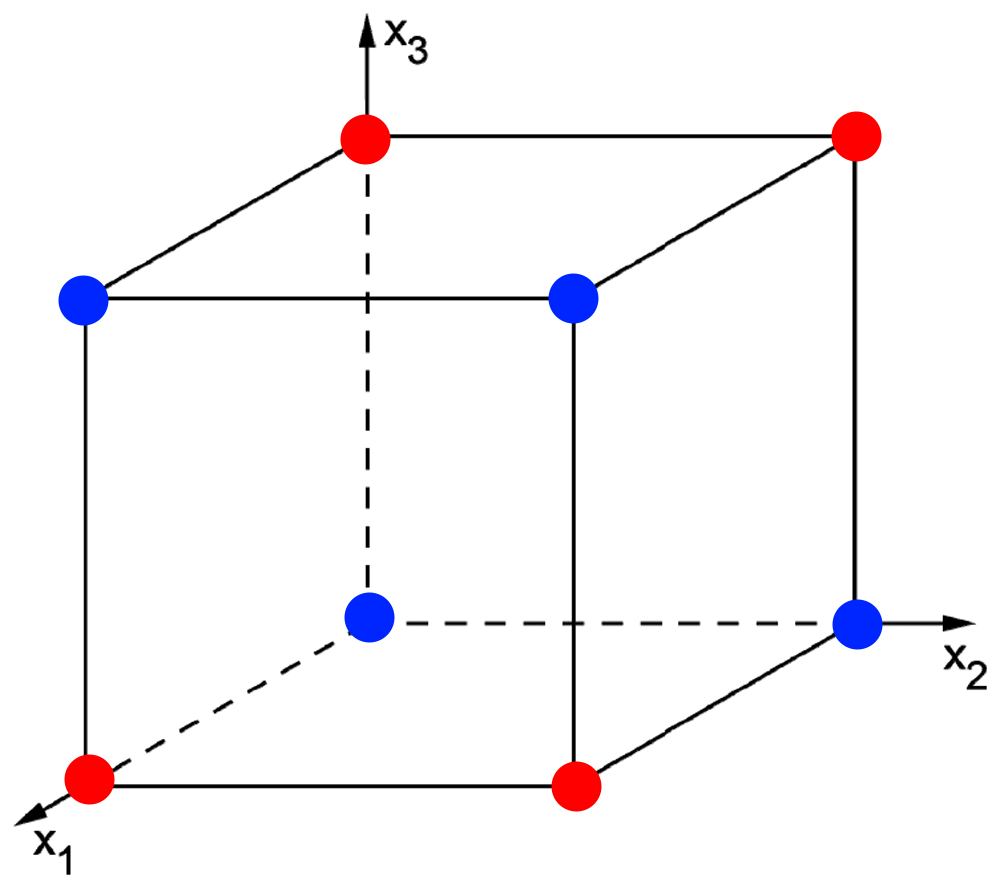
\includegraphics[width=80mm,scale=0.5]{khrapchenkos1.png}
        \caption{$A\otimes B$ Beispiel}
    \end{figure}
\end{frame}

\begin{frame}
    \begin{block}{Lemma}
        Ein monochromes Unterrechteck von $A \times B$ der Größe $s \times t$ kann maximal $\sqrt{st}$ Elemente von $A \otimes B$ überdecken.
    \end{block}
\end{frame}

\begin{frame}[t]
    Beweis:
    \newline
    \newline
    Sei $S\times T \subset A\times B$ ein Unterrechteck, $S\times T$ monochrom, $|S| = s, |T| = t$.
    \newline
    \newline
    Die Monochromie besagt, dass $\exists i: a_i \neq b_i\ \forall (a,b)\in S\times T$.
    \newline
    \newline
    Falls $(a,b) \in A\otimes B$, dann unterscheiden sich $a$ und $b$ in genau einem Index.
    \newline
    \newline
    Für die Überdeckung folgt also
    \[
        \min \{ |S|, |T|\} = \min \{ s, t\} \leq \sqrt{st}
    \]
    \hfill$\square$
\end{frame}

\begin{frame}
    \begin{block}{Theorem [Khrapchenko 1971]}
        Sei $f$ eine boolsche Funktion, die das Rechteck $A \times B$ separiert. Dann gilt:
        \[
            L(f) \geq \frac{\vert A \otimes B\vert ^2}{\vert A \vert\cdot\vert B\vert}
        \]
    \end{block}
\end{frame}

\begin{frame}[t]
    Beweis:
    \newline
    Sei $S_i\times T_i$ eine Zerlegung von $A\times B$ in $r$ monochrome Rechtecke, $i=1,\ldots,r$ mit $|S_i| = s_i$ und $|T_i| = t_i$.
    \newline
    Sei $c_i$ die Anzahl der Elemente aus $A\otimes B$ in $S_i\times T_i$.
    \newline
    \pause
    Aus dem obigem Lemma folgt: $c_i^2 \leq s_it_i$.
    \newline
    Da $S_i\times T_i$ eine paarweise disjunkte Zerlegung ist folgt
    \[
        |A\otimes B| = \sum\limits_{i=1}^r c_i, \hspace{1cm} |A\times B| = \sum\limits_{i=1}^r s_it_i
    \]
    \pause
    Es folgt:
    \[
        |A\otimes B|^2 = (\sum\limits_{i=1}^r c_i)^2 \leq
        r(\sum\limits_{i=1}^r c_i^2) \leq r(\sum\limits_{i=1}^r s_it_i) = r|A\times B|
    \]
    \pause
    \[
        \Rightarrow L(f) \geq \chi(f) = r \geq \frac{|A\otimes B|^2}{|A\times B|} = \frac{|A\otimes B|^2}{|A|\cdot|B|}
    \]
\end{frame}

\begin{frame}
    \begin{block}{Theorem}
        Sei
        \[
            \oplus_n := x_1 \oplus \dots \oplus x_n
        \]
        Dann folgt aus Kharapchenko's Theorem, dass
        \[
            L(\oplus_n) \geq n^2
        \]
    \end{block}
\end{frame}

\begin{frame}[t]
    Beweis:
    \newline
    \newline
    $A$ die Menge aller Vektoren mit ungerader Anzahl an Einsen.
    \newline
    Sei $B$ die Menge aller Vektoren mit gerader Anzahl an Einsen.
    \pause
    \newline
    Dann
    \[
        |A| = 2^{n-1}, |B| = 2^{n-1}, |A\otimes B| = n2^{n-1}
    \]
    \pause
    Es folgt
    \[
        L(\oplus_n) \geq \frac{n^2 2^{2(n-1)}}{2^{n-1}2^{n-1}} = n^2
    \]
    \hfill $\square$
\end{frame}

\begin{frame}
    \begin{block}{Theorem [Yablonskii 1954]}
        Sei $n \in \mathbb{N}$ mit $n \geq 2$. Dann
        \[
            L(\oplus_n) \leq 3np_n - 2p_n^2 \leq \frac{9}{8}n^2,
        \]
        wobei $p_n = 2^{\lfloor log_2n\rfloor}$.
        \newline
        \newline
        Wenn $n$ eine Zweierpotenz ist, dann gilt
        \[
            L(\oplus_n) = n^2
        \]
        \newline
        \newline
        Es wird vermutet, dass diese Schranke scharf ist.
    \end{block}
\end{frame}

\begin{frame}[t]
    Beweis:
    \newline
    \newline
    Sei $\lambda(n) := L(\oplus_n)$. 
    \newline
    Zudem sei $m := \lfloor \log_2 n \rfloor$, so dass $n = 2^m + k, 0 \leq k < 2^m$.
    \newline
    \newline
    \pause
    Zu zeigen: $\lambda(n) \leq 2^{2m} + 3k2^m = 3n p_n - 2 p_n^2$.
    \newline
    \newline
    \pause
    Beweis durch Induktion über $n = 2^m + k$. 
    \newline
    \newline
    Induktionsanfang: $n = 1 = 2^0 + 0$:
    \pause
    \[
        2^{2 \cdot 0} + 3 \cdot 0 \cdot 2^0 = 1 = \lambda(1) 
    \]
    und analog für 2.
\end{frame}{}

\begin{frame}[t]
    Induktionsschritt:
    \newline
    \newline
    Hierfür nutzen wir, dass für Funktionen $g,h$ gilt, dass
    \[
        f = g \oplus h \Leftrightarrow f = (g \land \lnot h) \lor (\lnot g \land h)
    \]
    Somit muss gelten, dass
    \[
        L(f) \leq 2L(g) + 2L(h)
    \]
    Somit erhalten wir
    \begin{alignat*}{1}
        &\lambda(n) \leq 2(\lambda(\lfloor n/2 \rfloor) + \lambda(\lceil n/2 \rceil)) = 3np_n - 2p_n^2 \leq \frac{9}{8} n^2
    \end{alignat*}
    \hfill$\square$
\end{frame}

\begin{frame}
    \begin{block}{Resultat}
        Nach den beiden obigen Lemmas folgt:
        \[
            n^2 \leq L(\oplus_n) \leq \frac{9}{8}n^2
        \]
        Für $n = 2^k$ gilt:
        \[
            n^2 = L(\oplus_n)
        \]
    \end{block}
\end{frame}

\begin{frame}
    \begin{block}{Theorem}
        \[
            L(Th^n_k) \geq k(n-k+1)
        \]
    \end{block}
\end{frame}

\begin{frame}[t]
    Beweis:
    \newline
    \newline
    $A$ sei die Menge aller Vektoren mit genau $k$ Einsen.
    \newline
    \newline
    \pause
    $B$ sei die Menge aller Vektoren mit genau $k-1$ Einsen.
    \newline
    \newline
    \pause
    Es folgt:
    \[
        |A\otimes B| = k|A| = (n-k+1)|B|
    \]
    \pause
    Somit
    \[
        L(Th_k^n) \geq \frac{(n-k+1)|A|\cdot k|B|}{|A|\cdot|B|} = k(n-k+1)
    \]
\end{frame}

%%%%%%%%%%%%%%%%%%%%%%%%%%%%%%%%%%%%%%%%%%%%%%%%%%%%%%%%%%%%%%%%%%%%%%
%\begin{frame}
%    \begin{block}{Theorem [Karchmer und Wigderson 1990]}
%        Sei $f$ eine boolsche Funktion, $A \subset f^{-1}(0)$ und $B %\subset f^{-1}(1)$, dann gilt:
%        \[
%            D(f) \geq \log \frac{\vert A \otimes B\vert ^2}{\vert A %\vert\cdot\vert B\vert}
%        \]
%    \end{block}
%\end{frame}
%
%\begin{frame}[t]
%    Beweis:
%    \newline
%    \begin{itemize}
%       \item (Karchmer und Widgerson) $D(f) = c(f)$
%        \item $c(f)$ beschreibt die Komplexität eines %Kommunikationsspiels
%    \end{itemize}
%    \pause
%    Wir spielen das folgende Spiel:
%    \begin{itemize}
%        \item Alice und Bob bekommen Informationen aus $a\in A$ resp. %$b\in B$.
%        \item Sie versuchen einen Index $i$ zu finden mit $a_i \neq %b_i$.
%        \item Wie viele Bits müssen sie dazu kommunizieren?
%    \end{itemize}
%\end{frame}
%
%\begin{frame}[t]
%    Beweis:
%    \newline
%    \newline
%    Sei $Y := A\otimes B$. Wir betrachten $Y$ als einen bipartierten %Graphen.
%   \newline
%    \newline
%    \pause
%    $N(v)$ sei die Menge aller Nachbarn von $v\in Y$, $d(v) = %|N(v)|$.
%   \newline
%    \newline
%    \pause
%    Für jedes $(a,b) \in A\times B$ sei $A(a,b)$ die Anzahl der Bits, %die Alice and Bob sendet und $B(a,b)$ die Anzahl der Bits, die Bob an %Alice sendet.
%    \newline
%    \newline
%    Es gilt dann
%    \[
%        A(a,b) \geq \log d(b), B(a,b) \geq log d(a)
%    \]
%    \pause
%    $C(a,b)$ sei die Anzahl der gesammten Bits, die versendet worden.
%\end{frame}
%
%\begin{frame}[t]
%    Beweis:
%    \newline
%    Sei $(a,b) \in Y$ gleichverteilt ausgewählt, dann folgt:
%    \begin{align*}
%        \mathbb{E} (C(a,b)) &= \frac{1}{|Y|} \sum\limits_{(a,b) \in %Y}^{} (A(a,b) + B(a,b)) \\
%        &= \frac{1}{|Y|} \sum\limits_{b \in B}^{} \sum\limits_{a\in %N(b)}^{} A(a,b) + \frac{1}{|Y|} \sum\limits_{a \in A}^{} %\sum\limits_{b\in N(a)}^{} B(a,b) \\
%        &\geq \frac{1}{|Y|} \sum\limits_{b \in B}^{} d(b)\log d(b) + %\frac{1}{|Y|} \sum\limits_{a \in A}^{} d(a)\log d(a) \\
%        &\geq \log \frac{|Y|}{|B|} + \log\frac{|Y|}{|A|} = \log 5\frac{|Y|^2}{|A||B|}
%    \end{align*}
%    Da $f(x) = x\log x$ konvex und somit nach der Jensen's %Ungleichung gilt:
%   \[
%        \frac{|B|}{|Y|} \sum\limits_{b\in B} \frac{1}{|B|} d(b) \log %d(b) 
%        \geq \frac{|B|}{|Y|} \frac{|Y|}{|B|} \log (\sum\limits_{b\in %B} \frac{1}{|B|} d(b) )
%    \]
%\end{frame}
%%%%%%%%%%%%%%%%%%%%%%%%%%%%%%%%%%%%%%%%%%%%%%%%%%%%%%%%%%%%%%%%%%%%%%

%%%%%%%%%%%%%%%%%%%%%%%%%%%%%%%%%%%%%%%%%%%%%%%%%%%%%%%%%%%%%%%%%%%%%%%%%%%%%%%%%%%%%%%%%%%%%%%%%%%%%%%%%%%%%%%%%%%%%%%%%%%%%%%%
